\documentclass{jarticle}
\usepackage{psfrag}
\pagestyle{empty}

\begin{document}
%%dvips(k) -Ppdf -E $B$$$C$?$s(B EPS $B$K$7$F$+$i!$$=$l$r%a%$%s$N(B LaTeX $B%U%!%$%k$KA^F~(B
\psfragscanon
\psfrag{s}[][]{$\theta$}
\psfrag{srad}[][]{$\theta$ [rad]}
\psfrag{1}[][]{$1$}
\psfrag{x}[][]{$x$}
\psfrag{y}[][]{$y$}
\resizebox{5cm}{!}{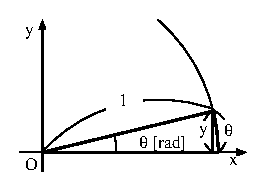
\includegraphics{small-sin.eps}}

\end{document}
